\cleardoublepage
\chapter{Preliminaries}

\todo{Why's the prefix needed for static analysis? => Is it because of the graph representation? (with a prefix, the visibility relation becomes transitive). See the robustness paper. Should we mention what robustness is? Then, the justification for our protocol is that it's the first PSI/NMSI impl amenable to analyse with robustness in mind.}

We begin with an introduction to the notation and basic concepts used throughout this thesis. We also review several \emph{strong} and \emph{weak} consistency models, based on the anomalies that are observable in each model. Finally, we discuss several protocols implementing some of these models, representing the previous work against which we compare our approach.

\section{Notation}

In this section, we define the elements we use throughout this chapter, such as transactions, histories, and relations. We follow the models used by Saeida Ardekani~\citep{ardekani_thesis}, Adya~\citep{adya_thesis} and Bernstein et al.~\citep{bernstein_concurrency}.

\subsection{Objects and Transactions}

We consider a database storing \textbf{\em objects} $\Obj = \{x, y, \ldots\}$, which we assume to be integer-valued. Clients interact with the database via \textbf{\em transactions} $\Trans = \{\tx_i \mid i \in \mathbb{N}\}$, with $i$ being the \emph{transaction identifier} of $\tx$. A transaction is a totally ordered sequence of read or write operations, followed by a \emph{terminating} operation: either commit or abort. This order follows the order in which the client invoked such operations. Given an object $x$ and a transaction $\tx_i$, we call $x_i$ to the \textbf{\em version} $i$ of $x$ written by $\tx_i$. We denote by $w_i(x_i)$ when a transaction $\tx_i$ writes a version $i$ of $x$, and $r_i(x_i)$ when $\tx_i$ reads a version $i$ of $x$. Finally, we denote by $c_i$ when $\tx_i$ commits, and $a_i$ when it aborts. We assume an initial transaction $\tx_0$ writes the initial versions of every object in the database. Without loss of generality, we also assume that no transaction performs \emph{blind updates}, that is, for every write operation $w_i(x_i)$ performed by $\tx_i$, there's always a preceding read operation $r_i(x_i)$. We say that a transaction is \textbf{\em read-only} if its set of operations does not include writes, and \textbf{\em update} otherwise.

\subsection{Histories}
\label{sect:histories}

We call a \textbf{\em history} $h$ to the finite set of all transactions with disjoint identifiers issued against a database. We denote the set of all possible histories by $\Hist$. For some history $h$, $\hb_h$ denotes a \textbf{\em happens-before} strict partial order over $h$, such that for any two transactions $\tx_i$ and $\tx_j$, if $w_i(x_i)$ and $r_j(x_i)$, $\tx_i \hb_h \tx_j$ (that is, $\tx_j$ reads the version $i$ of $x$ written by $\tx_i$). Intuitively $\tx_i \hb_h \tx_j$ means that $\tx_j$ is aware of the updates performed by $\tx_i$, and thus the outcome of the operations in $\tx_j$ may depend on the effects of $\tx_i$. In this case, we say that $\tx_i$ is a \textbf{\em causal dependency} of $\tx_j$. A transaction $\tx_i$ is \textbf{\em pending} in $h$ if $(c_i \vee a_i) \notin h$. We can represent the history and the relations between operations and transactions as a graph, following Bernstein et al~\citep{bernstein_concurrency}.

\begin{figure}[h]
  \centering
  \vspace{-0.4cm}
  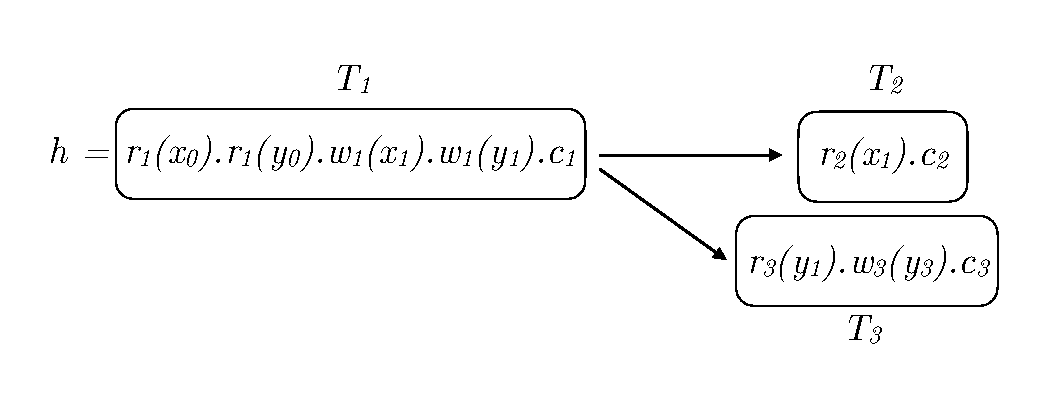
\includegraphics[width=0.7\textwidth]{figures/history.pdf}
  \vspace{-1cm}
  \caption{Example of history represented as a graph. Arrows represent the causal dependencies between operations. Adapted from \em{Saeida Ardekani~\citep{ardekani_thesis}}.}
  \label{fig:history}
\end{figure}

Figure~\ref{fig:history} above shows an example, with $\tx_1 \hb_h \tx_3$ and $\tx_1 \hb_h \tx_2$. We say that two transactions $\tx_i$ and $\tx_j$ are \textbf{\em concurrent} in $h$ (denoted by $\tx_i \parallel \tx_j$) if neither $\tx_i \hb_h \tx_j$ nor $\tx_j \hb_h \tx_j$. In the figure above, $\tx_2$ and $\tx_3$ are concurrent.

\todo{Introduce distributed system here? Or is it covered in chapter 1?}

\section{Consistency Models}

In this section, we define what a consistency model is, distinguishing between \emph{strong} and \emph{weak} models. We give an overview of several models, and compare them in terms of their undesirable effects.

We define a consistency model as a set of histories $\Cons$, such that $\Cons \subseteq \Hist$. Intuitively, a consistency model \emph{constrains} the set of possible histories by specifying how operations interleave in any given history. We say that a given history $h$ \emph{satisfies} a consistency model $\Cons$ if $h \in \Cons$, and that $h$ \emph{violates} $\Cons$.

In the context of databases, the definition of a consistency model maps to the concept of an \emph{isolation level} (I in AC\underline{I}D), which specifies the degree to which concurrent transactions in a database are aware of each other~\citep{adya_thesis}. We use the term consistency throughout this thesis, in accordance with Adya~\citep{adya_thesis}.

Traditionally, the different consistency models have been defined in terms of \emph{anomalies}~\citep{sql-critique}, that map to a set of undesirable histories that are observable by the system. Intuitively, we can distinguish between \emph{strong} and \emph{weak} consistency models depending on the number of anomalies they disallow, with stronger models restricting the set of possible histories more than weak ones. In the sections that follow, we give a brief overview of the traditional anomalies following the definitions advanced by Berenson et al.~\citep{sql-critique}, as well as different consistency models that preclude them. % Figure~\ref{fig:anomalies} shows a quick summary of the models and anomalies we cover.

% \begin{figure}[h]
% \begin{center}
% \begin{tabularx}{\linewidth}{ >{\centering}p{8cm} | *{5}{>{\centering}X}}
%     \multirow{2}{*}{\em Anomalies} & \multicolumn{5}{c}{Consistency Models} \tabularnewline \cline{2-6}
%     & SER & SI & PSI & NMSI & RC \tabularnewline \hline
%     Dirty Write & x & x & x & x & x \tabularnewline
%     Dirty Read & x & x & x & x & x \tabularnewline
%     \hline % Distinguish between ACID or not
%     Non-Repeatable Read & x & x & x & x & \checkmark \tabularnewline
%     Lost Update & x & x & x & x & \checkmark \tabularnewline
%     \hline % Distinguish between weak and strong
%     Write Skew & x & \checkmark & \checkmark & \checkmark & \checkmark \tabularnewline
%     Long Fork & x & x & \checkmark & \checkmark & \checkmark \tabularnewline
% \end{tabularx}
% \end{center}
% \caption{Anomaly Comparison of Consistency Models \emph{(x}:disallowed, \checkmark:allowed\emph{)}. Adapted from \em{Saeida Ardekani et al.~\citep{ardekani-nsmi}}.}
% \label{fig:anomalies}
% \end{figure}

\begin{definition}[Dirty Write]
A \emph{Dirty Write} occurs in a history $h$ when a transaction $\tx_i$ modifies an object $x$ that was previously modified by another pending transaction $\tx_j$. If any of the two transactions commit or abort, it is not clear what value the object $x$ should have. A Dirty Write can be represented by a history such as $w_1(x_1).w_2(x_2).(c_1 \vee a_1).(c_2 \vee a_2)$, where the termination order of the transactions can be arbitrary. The anomaly occurs even if any of the transactions aborts.
\end{definition}

\begin{definition}[Dirty Read]
A \emph{Dirty Read} occurs in a history $h$ when a transaction $\tx_i$ reads an object $x$ modified by a pending transaction $\tx_j$. If $\tx_j$ ultimately aborts in $h$, the value observed by a $\tx_i$ was never supposed to occur in $h$. This is represented by a history such as $r_1(x_0)\ldots w_1(x_1)\ldots r_2(x_1)\ldots c_2\ldots a_1$.
\end{definition}

Both of these anomalies can be prevented by making a transaction's changes visible only after it commits. For example, updates can be buffered locally in the context of a transaction. All the consistency models we describe in the sections that follow preclude dirty writes and reads. Transactions executing under such models offer \emph{atomicity} (A in \underline{A}CID).

\begin{definition}[Non-Repeatable Read]
A non-repeatable read---also called a \emph{fuzzy read}--occurs whenever a transaction $\tx_i$ observes different values for an object $x$ on subsequent read operations when interleaved by a commit by another transaction, $\tx_j$. This can be seen in $r_1(x_0)\ldots r_2(x_0).w_2(x_2).c_2 \ldots r_1(x_2)$. Here, $\tx_1$ observers two different values of $x$: the initial version $x_0$ and the version $x_2$ written by $\tx_2$.
\end{definition}

The non-repeatable read anomaly can also be prevented in an easy way: a transaction can keep a cache of already read values. Subsequent read operations can return values from this read cache.

\begin{definition}[Lost Update]
A \emph{Lost Update} occurs in a history $h$ when two concurrent transactions update the same object $x$ and successfully commit. In this case, the update written by whichever transaction commits first is ``lost'' after the second transaction commits. This can be seen in a history such as $r_1(x_0)\ldots r_2(x_0).w_2(x_2) \ldots w_1(x_1).c_1\ldots c_2$. After $\tx_2$ commits, version $x_1$ is no longer visible to subsequent transactions.
\end{definition}

For the purposes of this thesis, and following the definition used by Saeida Ardekani~\citep{ardekani_thesis}, we say that a consistency model is \emph{strong} if it prevents concurrent transactions to modify the same object. That is to say, a strong consistency model preclude dirty writes and reads, along with lost update anomaly. A model that allows concurrent transactions to modify the same object is \emph{weak}.

We now review several well-known strong consistency models, along with a weak model that will serve as a baseline comparison in the following chapters.

\subsection{Serialisability (SER)}

Serialisability restricts the set of possible histories to those equivalent to some \emph{serial} execution. That is to say, under a traditional system offering Serialisability, the happens-before relation we introduced in~\ref{sect:histories} is strengthened with a \emph{strict total order} over the transactions in a history \todo{does it need to be strict?}. A history such as the one in Figure~\ref{fig:history} is serialisable, because we can order $\tx_2$ to occur before $\tx_3$ (or vice versa); while the one depicted in Figure~\ref{fig:non_ser_history} is not.

\begin{figure}[h]
  \centering
  \vspace{-0.3cm}
  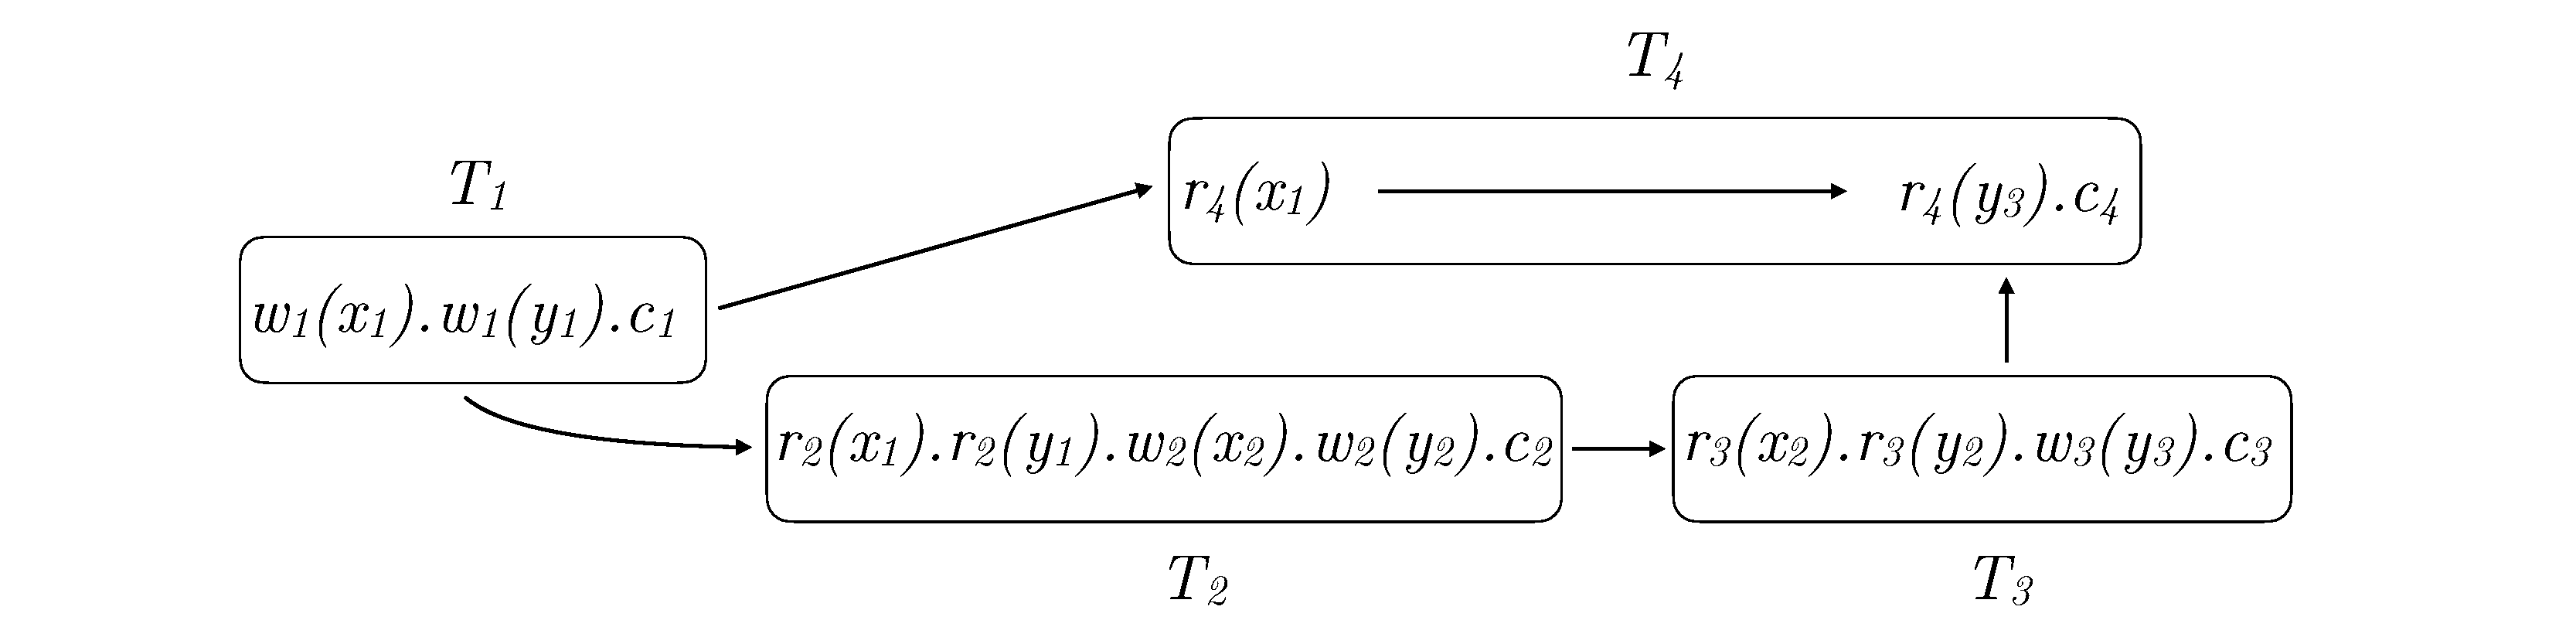
\includegraphics[width=\textwidth]{figures/non_ser_hist.pdf}
  \vspace{-1cm}
  \caption{Example of a non-serialisable history. $\tx_4$ observes version $y_3$ written by $\tx_3$, but fails to observe version $x_2$ written by $\tx_1$. This result can't be obtained by executing the transactions in any sequence, and thus the history is not serialisable.}
  \label{fig:non_ser_history}
\end{figure}

\todo{Mention something about serial order being hard to achieve in a distributed setting?}

\subsection{Snapshot Isolation (SI)}
\label{sect:si}

Proposed by Berenson et al.~\citep{sql-critique}, Snapshot Isolation (SI) relaxes the total ordering guarantees of Serialisability by requiring only a partial order among committed transactions. To preclude the Lost Update anomaly, SI introduces the concept of a \emph{snapshot}: a private view of the data written by committed transactions. This snapshot is created at the time the transaction starts, called its \emph{start timestamp}. A transaction $\tx$ is not able to see updates made by other transactions that commit after $\tx$'s start timestamp. When a transaction $\tx$ is ready to commit, it gets assigned a \emph{commit timestamp}, larger than any previous start or commit timestamp. Transaction $\tx$ commits successfully only if no other concurrent transaction updated the same objects as $\tx$. Under SI, two transactions are concurrent if their start-commit timestamps intervals overlap, and read-only transactions always commit. When two transactions update a non-disjoint set of objects, we say they \textbf{\em write-conflict}.

Due to partial ordering among committed transactions, along with the condition that concurrent transactions only abort if their set of updated objects overlap, a system under Snapshot Isolation is able observe the so-called \emph{Write Skew} anomaly. This anomaly occurs when an external invariant is violated as a result of concurrent non-conflicting transactions. As an example, suppose that objects $x$ and $y$ are related by a constraint such that $x + y \le 10$, with $x = 5$ and $y = 2$ as the initial state. In such a setting, a history such as the following can violate the invariant: $h = r_1(x=5).r_1(y=2).r_2(x=5).r_2(y=2).w_1(x=7).w_2(y=4).c_1.c_2$. Both $\tx_1$ and $\tx_2$ start their execution and observe a consistent state that upholds the invariant. Then, $\tx_1$ updates the object $x$ to the value $7$, which still maintains the invariant, as $7 + 2 \le 10$. Concurrently, $\tx_2$ proceeds as $\tx_1$, updating $y$ to $4$, which also maintains the original invariant ($5 + 4 \le 10$). However, as the result of both $\tx_1$ and $\tx_2$ successfully committing, the invariant is violated, with $7 + 4 \not\le 10$.

%  Figure~\ref{fig:write_skew_history} shows an example of such a history.

% Reads and updates are performed against the transaction snapshot (precluding non-repeatable reads) and made visible after the transaction commits (precluding dirty reads and writes).

% \begin{figure}[h]
%   \centering
%   \vspace{-0.4cm}
%   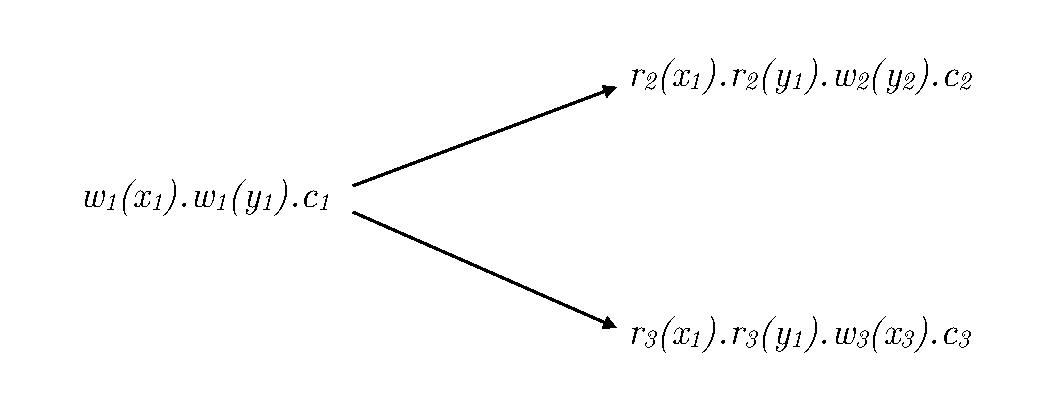
\includegraphics[width=0.6\textwidth]{figures/skew_history.pdf}
%   \vspace{-0.6cm}
%   \caption{Example of a history showing the write skew anomaly. Both $\tx_2$ and $\tx_3$ observe a consistent state of objects $x$ and $y$, but the versions diverge after both transactions commit.}
%   \label{fig:write_skew_history}
% \end{figure}

\begin{definition}[Write Skew]\todo{Revise}
A \emph{Write Skew} occurs whenever two non-conflicting transactions update objects related with an external invariant, successfully commit, and as a result violate the original invariant.
\end{definition}

\todo{Limitations?}

\subsection{Parallel Snapshot Isolation (PSI)}

% From Sovran:
% Snapshot isolation is inadequate for a system replicated at many sites, due to two issues. First, to define snapshots, snapshot isolation imposes a total ordering of the commit time of all transactions, even those that do not conflict. Establishing such an ordering when transactions execute at different sites is inefficient. Second, the writes of a committed transaction must be immediately visible to later transactions. Therefore a transaction can commit only after its writes have been propagated to all remote replicas, thereby precluding asynchronous propagation of its updates.

Parallel Snapshot Isolation (PSI), proposed by Sovran et al.~\citep{psi-intro}, relaxes some of the guarantees offered by classical Snapshot Isolation. Recall from section~\ref{sect:si} that transactions in a system offering SI require monotonically-increasing \emph{start} and \emph{commit} timestamps. The presence of these timestamps require the system to maintain a total order among the commit time of transactions: a so-called total \textbf{\em commit order}. Total order guarantees are challenging to scale in the context of geographically replicated systems, which becomes the principal motivation for the introduction of Parallel Snapshot Isolation. Non-conflicting transactions executing under PSI are allowed to exhibit a relative commit order that varies between replicas. Conflicting transactions are not allowed, as in Snapshot Isolation.

Allowing different commit orderings for non-conflicting transactions at different replicas (or \emph{sites}) makes PSI susceptible to the \emph{Long Fork} anomaly~\citep{psi-intro}. Consider the history depicted in Figure~\ref{fig:long_fork_history}. If transactions $\tx_3$ and $\tx_4$ are executing in different sites, they might observe different commit orderings for $\tx_1$ and $\tx_3$.

\begin{figure}[h]
  \centering
  \vspace{-0.5cm}
  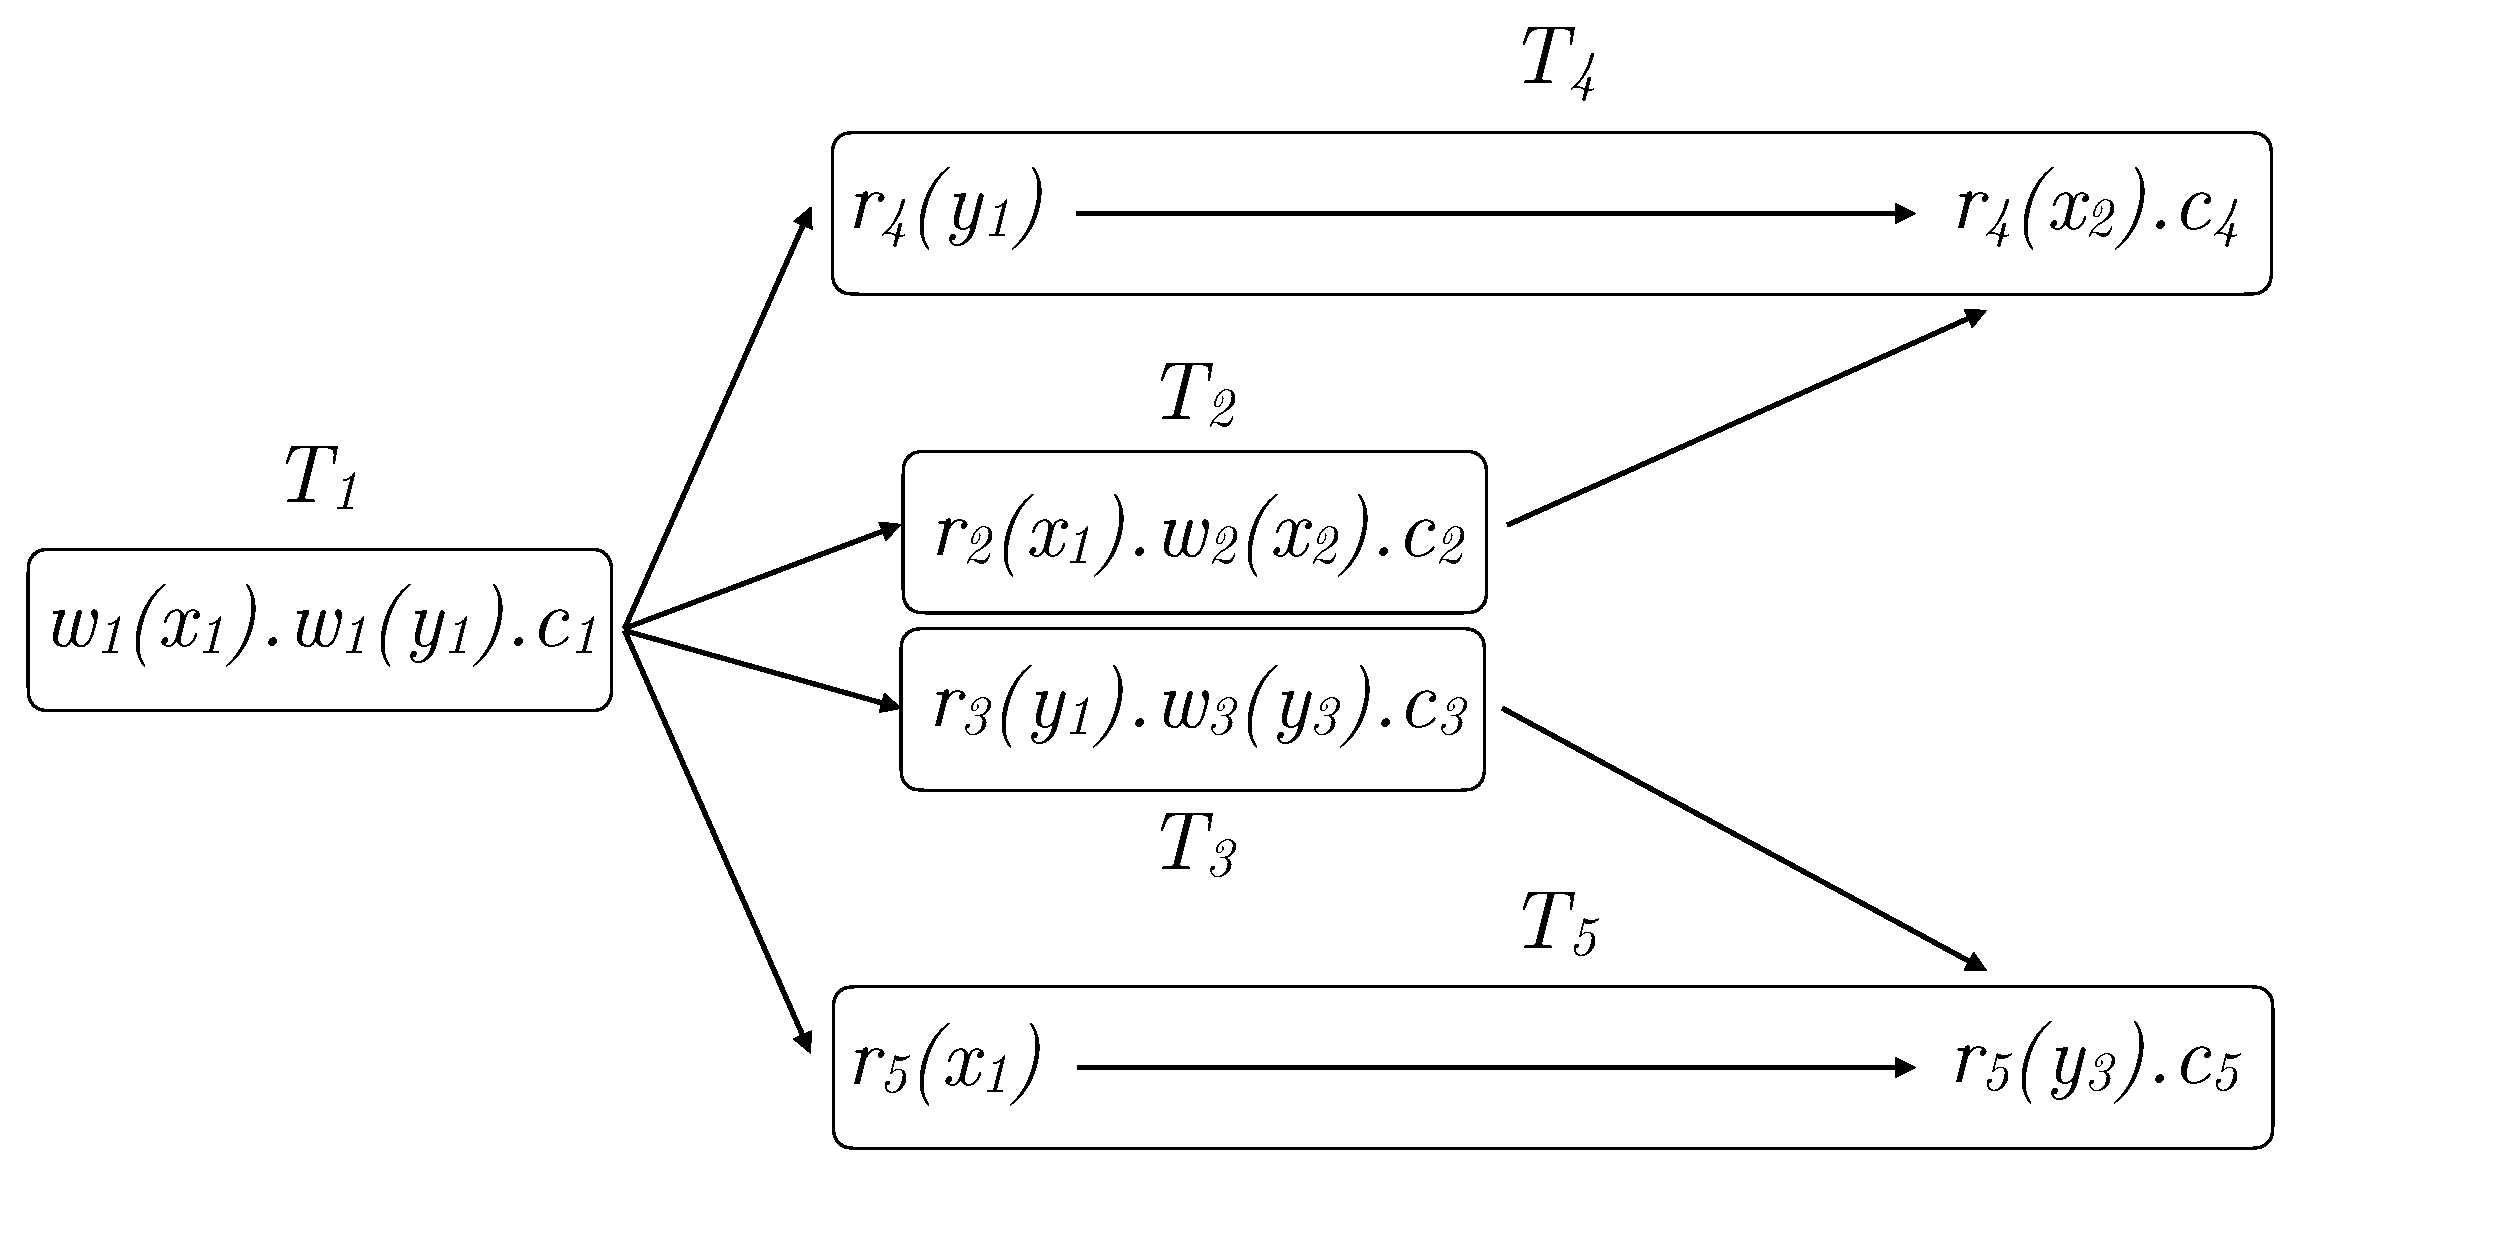
\includegraphics[width=0.7\textwidth]{figures/long_fork_hist.pdf}
  \vspace{-0.5cm}
  \caption{Example of a history showing the long fork anomaly. Transaction $\tx_3$ observes $\tx_1 \rightarrow \tx_2$ while $\tx_4$ observes $\tx_2 \rightarrow \tx_1$. Adapted from \em{Saeida Ardekani~\citep{ardekani_thesis}}.}
  \label{fig:long_fork_history}
\end{figure}

\begin{definition}[Long Fork]
A \emph{Long Fork} occurs whenever a transaction is able to observe different orderings of previous non-conflicting update transactions.
\end{definition}

\todo{Mention causal ordering while replicating?}

\subsection{Non-Monotonic Snapshot Isolation (NMSI)}

\todo{Specification of NMSI (PSI timestamp is fixed at tx.start() time (base freshness), which causes stale transactions in geo-replicated settings.) How big of a deal are anomalies in the applications that we target?}

\todo{From \textit{Making PSI serialisable}: Saeida Ardekani et al. have proposed a variant of PSI called non-monotonic snapshot isolation (NMSI). It is possible to prove that PSI and NMSI produce the same set of anomalies, provided that database clients cannot observe the real-time order between operations: the difference between them lies only in the concurrency control algorithm used. Hence, our results are equally applicable to NMSI.}

\subsection{Read Committed (RC)}

Read Committed is the weakest protocol that satisfies the atomicity guarantee of transactions, by preventing dirty reads and writes. Although this model specifies that all or none of the updates by a transaction are applied to the database, it does not prevent concurrent transactions from observing only a subset of those updates. In this thesis, we use Read Committed as a baseline against which we compare the protocols we implement. \todo{Anything else?}

\subsection{Anomaly Comparison}

Figure~\ref{fig:anomalies} summarises the consistency models we reviewed together with the anomalies that they allow.

\begin{figure}[h]
\begin{center}
\begin{tabularx}{\linewidth}{ >{\centering}p{8cm} | *{5}{>{\centering}X}}
    \multirow{2}{*}{\em Anomalies} & \multicolumn{5}{c}{Consistency Models} \tabularnewline \cline{2-6}
    & SER & SI & PSI & NMSI & RC \tabularnewline \hline
    Dirty Write & x & x & x & x & x \tabularnewline
    Dirty Read & x & x & x & x & x \tabularnewline
    \hline % Distinguish between ACID or not
    Non-Repeatable Read & x & x & x & x & \checkmark \tabularnewline
    Lost Update & x & x & x & x & \checkmark \tabularnewline
    \hline % Distinguish between weak and strong
    Write Skew & x & \checkmark & \checkmark & \checkmark & \checkmark \tabularnewline
    Long Fork & x & x & \checkmark & \checkmark & \checkmark \tabularnewline
\end{tabularx}
\end{center}
\caption{Anomaly Comparison of Consistency Models \emph{(x}:disallowed, \checkmark:allowed\emph{)}. Adapted from \em{Saeida Ardekani et al.~\citep{ardekani-nsmi}}.}
\label{fig:anomalies}
\end{figure}

\section{Catalog of Protocols}
\subsection{Walter}
\subsection{Jessy}
% \subsection{GMU} Tentative, since we don't talk about US in previous section
